% This is samplepaper.tex, a sample chapter demonstrating the
% LLNCS macro package for Springer Computer Science proceedings;
% Version 2.20 of 2017/10/04
%
\documentclass[runningheads]{llncs}
%
\usepackage{graphicx}
\usepackage{mathtools,amssymb}
% Used for displaying a sample figure. If possible, figure files should
% be included in EPS format.
%
% If you use the hyperref package, please uncomment the following line
% to display URLs in blue roman font according to Springer's eBook style:
% \renewcommand\UrlFont{\color{blue}\rmfamily}

\begin{document}
%
\title{Parallel Computations for Various Scalarization Schemes in Multicriteria Optimization Problems\thanks{This research was supported by the Russian Science Foundation, project No 16-11-10150 ''Novel efficient methods and software tools for time-consuming decision making problems using supercomputers of superior performance.''}}
%
\titlerunning{Parallel Computations in Multicriteria Optimization}
% If the paper title is too long for the running head, you can set
% an abbreviated paper title here
%
\author{Victor Gergel\orcidID{0000-0002-4013-2329} \and Evgeny Kozinov \orcidID{0000-0001-6776-0096}}

\authorrunning{V. Gergel et al.} % if too long for running head
% First names are abbreviated in the running head.
% If there are more than two authors, 'et al.' is used.
%
\institute{Lobachevsky State University of Nizhni Novgorod, Nizhni Novgorod, Russia \\
              \email{gergel@unn.ru, evgeny.kozinov@itmm.unn.ru}
}
%
\maketitle              % typeset the header of the contribution
%
\begin{abstract}
In the present paper, a novel approach to parallel computations for solving time-consuming multicriteria global optimization problems is presented. This approach includes various methods for the scalarization of vector criteria, dimensionality reduction with the use of the Peano space-filling curves, and efficient global search algorithms. The applied criteria scalarization methods can be altered in the course of computations in order to better meet the stated optimality requirements. To reduce the computational complexity of multicriteria problems, the methods  developed feature an extensive use of all the computed optimization information and are well parallelized for effective performance on high-performance computing systems. Numerical experiments confirmed the efficiency of the developed approach.

\keywords{Multicriteria optimization \and criteria scalarization \and global optimization \and parallel computations.}
\end{abstract}
%
%
%
\section{Introduction} \label{sec:1}
 
Multicriteria optimization (MCO) problems arise in various applications of science and technology. The wide scope of application of MCO problems determines the intensity of research in the field \cite{c1,c2,c3,c4,c5}.

Usually, the criteria of the MCO problems are contradictory, and obtaining the decisions, which provide the best values with respect to all criteria simultaneously, is impossible. In such situations, a set of efficient (non-dominated) decisions is considered for such MCO problems,  where the improvement of
the values of some criteria cannot be achieved without sacrificing the efficiency values with respect to other criteria. When solving MCO problems, it may become necessary to obtain the whole set of the efficient decisions (the Pareto set) that may require performing a large amount of computations. Besides, the analysis of a large set of the efficient decisions may appear to be
difficult for a decision maker. Therefore, in practice the finding of only a relatively small set of efficient decisions may be justified. Constructing such a limited set of efficient decisions is performed usually according to the optimality requirements defined by the decision-maker.

The restricted set of the computed efficient decisions leads to a notable reduction in the amount of required computations. However, the criteria of efficiency may have a complex multiextremal form, and the computation of the criteria values may appear to be time-consuming. One way to overcome the considerable computational complexity when solving MCO problems is to use high-performance supercomputing systems.

In the present paper, the research results on the development of highly efficient parallel methods of the multicriteria optimization using the search information obtained in the course of computations \cite{c6,c7,c8,c9,c16} are presented. A novel contribution consists in the development of an approach whereby it is possible to use different MCO problem criteria scalarization schemes taking into account different optimality requirements to desirable decisions. For the scalarization schemes considered in this study, a general method of parallel computations was proposed and the computational evaluation of the developed approach's efficiency was performed.

The further structure of the paper is as follows. In Section 2, the statement of the multicriteria optimization problems is given. In Section \ref{sec:3}, a general scalarization scheme for the MCO problem criteria involving various kinds of criteria convolution is proposed. In Section \ref{sec:4}, the search information obtained in the course of computations, which can be reused after the altering of the applied scalarization schemes, is considered. Also, this section presents a general scheme for the parallel execution of the global search algorithms, in the framework of which an efficient parallel method for solving time-consuming global optimization problems is considered. Section \ref{sec:5} contains the results of the numerical experiments confirming that the approach developed by the authors is quite promising. In the Conclusions section, the obtained results are discussed and possible main areas for further studies are outlined.

\section{Multicriteria optimization problem statement} \label{sec:2}

In the most general form, the multicriteria optimization problem is defined in the following way 
\begin{equation}
f(y) \to min, y \in D :g(y) \leq 0 ,
\label{eq:1}
\end{equation}
where $y=(y_1,y_2, \dots ,y_N)$ is a vector of varied parameters, \\$f(y)=(f_1 (y),f_2 (y), \dots ,f_s (y))$ is the vector of the efficiency criteria, $D \subset R^N$ is the search domain 
\begin{equation}
D = \{ y\in R^N:a_i \leq y_i \leq b_i, 1 \leq i \leq N \},
\label{eq:2}
\end{equation}
for given vectors $a$ and $b$, and $g(y)= (g_1 (y),g_2 (y), \dots ,g_m (y))$ are the constraints of the MCO problem (the conditions of feasibility of the chosen decisions $y \in D$).

In the most complex cases, the criteria $f_i (y)$, $1 \leq i \leq s$, can be multiextremal and computing the values of these ones can appear to be time-consuming. Usually, the criteria $f_i (y)$, $1 \leq i \leq s$, satisfy the Lipschitz condition 
\begin{equation}
|f_i (y_1 )-f_i (y_2 ) | \leq L_i \|y_1-y_2\|,1 \leq i \leq s,
\label{eq:3}
\end{equation}
where $L_i$ are the Lipschitz constants for the criteria $f_j (y)$, $1 \leq j \leq s$ and $\|*\|$ denotes the Euclidean norm in $R^N$. 

Without any loss in generality, in further consideration we will assume the criteria $f_i (y)$, $1 \leq i \leq s$ to be non-negative and their decrease corresponds to the increase in the efficiency of the chosen decisions. 


\section{Reducing multicriteria optimization to multiple
global search problems} \label{sec:3}

As mentioned above, for solving MCO problems it is required to find a set of the efficient (Pareto optimal) decisions, for which the values cannot be improved with respect to all criteria simultaneously. However, a large amount of computations may be required to  find a complete set of efficient decisions. A commonly used approach to reducing the computational costs consists in finding of only a relatively small set of efficient decisions, defined according to the optimality requirements of the decision maker. In many cases, the required decisions are found by means of reducing the vector criteria to some general scalar efficiency function that allows applying a variety of already existing global optimization methods for solving MCO problems. Possible scalarization methods include, for example, the weighted sum method, the compromise programming method, the weighted min-max method, as well as many other methods -- see, for example, \cite{c2,c4}. Within the developed approach, it was proposed to employ the following methods of scalarization of the vector criterion of MCO problems.

1. One of the widely applied scalarization methods consists in the use of the min-max convolution of the criteria \cite{c4,c6}:
\begin{equation}
\begin{split}
F_1 (\lambda,y)=\max{(\lambda_i f_i (y),1 \leq i \leq s)}, \\
\lambda=(\lambda_1,\lambda_2,\dots,\lambda_s)\in \Lambda \subset R^s: \sum_{i=1}^s{\lambda_i=1}, \lambda_i \geq 0, 1 \leq i \leq s.
\end{split}
\label{eq:4}
\end{equation}

2. In the case when the criteria can be arranged in the order of importance, the method of successive concessions (MSC) is usually applied \cite{c5,c6}. In this method, the multistage computations can be reduced to solving the following scalar optimization problem 
\begin{equation}
F_2(\delta,y)=f_s(y), f_i(y) \leq f_i^{min}+\delta_i (f_i^{max}- f_i^{min}), 1 \leq i < s, g(y) \leq 0,y \in D,
\label{eq:5}
\end{equation}
where $f_i^{min}$, $f_i^{max}$, $1 \leq i < s$, are the minimum and the maximum values of the criteria in the domain $D$ from (\ref{eq:2}), and $0 \leq \delta_i \leq 1$, $1 \leq i < s$, are the concessions with respect to each criterion. 

3. If an estimate of the criteria values for the required decision exists a \textit{priori} (for example, based on some ideal decision), the solution of a MCO problem can consist in finding an efficient decision that matches the predefined optimality values \cite{c2,c4}:
\begin{equation}
F_3 (\theta,y)= 1/s \sum_{i=1}^s{\theta_i(f_i(y)-f_i^*)^2 }, g(y) \leq 0, y \in D,
\label{eq:6}
\end{equation}
where $F_3 (\theta,y)$ is the mean square deviation of the decision $y \in D$ from the sought ideal decision $y^*$, and the values $0\leq \theta_i \leq 1$, $1 \leq i < s$, are the importance parameters of the approximation accuracy with respect to each variable $y_i$, $1 \leq i \leq N$.

In the general case, the statements of the global optimization problems generated by the criteria scalarization schemes (\ref{eq:4})-(\ref{eq:6}) can be represented in the form:
\begin{equation}
  \min\varphi(y)=\min{F(\alpha,y)},  g(y) \leq 0, y \in D, 
\label{eq:7}
\end{equation}
where $F$ is the objective function generated as a result of the criteria scalarization, $\alpha$ is the vector of parameters of the criteria convolution, $g(y)$ are the constraints of the MCO problem, and $D$ is the search domain from (\ref{eq:2}). It should be noted that due to the possibility of altering the optimality requirements in the course of computations, the form of the function $\varphi(y)$ from (\ref{eq:7}) can vary. Thus, it may be necessary to alter the scalarization method employed (\ref{eq:4})-(\ref{eq:6}) and/or to change the convolution parameters $\lambda$, $\delta$, and $\theta$. Such variations form a set of scalar global optimization problems
\begin{equation}
  \mathbb{F}_T=\{ F_k (\alpha_i,y): 1\leq i \leq T, k=1,2,3 \}.
\label{eq:9}
\end{equation}

This set of problems can be formed sequentially in the course of computations. The problems in this set can be solved either sequentially or simultaneously -- in the time sharing mode or in parallel with the use of high performance computational systems. The opportunity of forming the set $\mathbb{F}_T$ allows formulating \textit{a new class of multicriteria global optimization problems}.

Within the framework of the  proposed approach, one more step of transformation of the problems $F(\alpha,y)$ from the set $\mathbb{F}_T$ is applied -- namely, the dimensionality reduction with the use of the Peano space-filling curves (evolvents) $y(x)$ providing an unambiguous mapping of the interval $[0,1]$ onto an $N$-dimensional hypercube $D$ \cite{c10,c11}. As a result of such reduction, a multidimensional problem (\ref{eq:7}) is reduced to a one-dimensional global optimization problem:

\begin{equation}
F(\alpha,y(x^*)) = \min{\{F(\alpha,y(x)): g(y(x))\leq 0, x \in [0,1]\}}.
\label{eq:10}
\end{equation}

The dimensionality reduction allows applying many highly efficient\\ one-dimensional global search algorithms -- see, for example, \cite{c10,c11,c12,c14} -- for solving the problems of the set $\mathbb{F}_T$ from (\ref{eq:9}). It should be also noted that according to (\ref{eq:3}) the function $F(\alpha,y(x))$ satisfies the uniform H\"{o}lder condition with a constant $H$ \cite{c10,c11} i.e.
\begin{equation}
  |F(\alpha,y(x' )-F(\alpha,y(x'')|\leq H |x'-x''|^{1/N}.
\label{eq:11}
\end{equation}


\section{Parallel computations for solving multiple global optimization problems} \label{sec:4}

The numerical solving of the MCO problems consists usually in sequential computing of the values of the criteria $f(y)$ and the constraints $g(y)$ from (\ref{eq:1}) at the points $y^i$, $0 \leq i \leq k$, of the search domain $D$ \cite{c10,c12,c13,c14}. After the scalarization of the vector criterion (\ref{eq:7}) and the application of the dimensionality reduction (\ref{eq:10}), the obtained search information takes the form of the set:
\begin{equation}
  A_k=\{(x_i,z_i,f_i,g_i )^T:1 \leq i \leq k\},
\label{eq:12}
\end{equation}
where $x_i$, $1 \leq i \leq k$ are the reduced points of the executed global search iterations arranged in ascending order of the coordinates and $z_i$,  $f_i$, $g_i$, $1 \leq i \leq k$, are the values of the scalar criterion, the objective function criteria and the constraints respectively at these points for the current optimization problem $F(\alpha,y(x))$.

The availability of the set $A_k$ from (\ref{eq:12}) allows the transformation of the values of the criteria and constraints calculated earlier into the values of the current optimization problem $F(\alpha,y(x))$ from (\ref{eq:7}) without repeating the time-consuming computations of the values of criteria and constraints i. e.
\begin{equation}
  (x_i,f_i,g_i ) \to z_i = F(\alpha,y(x_i)) ,1 \leq i \leq k.
\label{eq:13}
\end{equation}

In this way, the whole search information $A_k$ from (\ref{eq:12}) recalculated according to (\ref{eq:13}) can be reused to continue the solution of the MCO problem. This can provide a considerable reduction of the amount of computations performed for solving every next MCO problem of the set $\mathbb{F}_T$ from (\ref{eq:9}) up to a limited number of global search iterations.

A further increase in computational efficiency when solving MCO problems can be provided by means of parallel computations. Within the framework of the developed approach, a general parallel computation scheme for solving global optimization problems is applied -- namely, parallel computations are provided by the simultaneous computing of the values of the minimized function $F(\alpha,y(x))$ from (\ref{eq:7}) at several different points of the search domain $D$ \cite{c6,c10}. Such an approach provides the parallelization of the most time-consuming part of the global search computations and can be applied to any global optimization method for a variety of global optimization problems.

The state-of-the-art in the field of global optimization is reviewed, for example, in \cite{c10,c12,c13}. In the present paper, the proposed approach is based on the information-statistical theory of global search \cite{c10}. This theory has been applied as a basis for the development of a large number of efficient methods of multiextremal optimization -- see, for example, \cite{c6,c7,c8,c9,c10,c11,c15,c16,c17,c18}. The main ideas of the algorithms developed consist in the dimensionality reduction with the use of the Peano space-filling curves and in parallel computations by simultaneous computing the values of the minimized functions at several points of the search domain. From the general point of view, the developed \textit{multidimensional parallel global search algorithms} (MPGSA) can be presented by a unified computation scheme as follows \cite{c6,c10,c15}.

Let $p>1$ be the number of the applied processors (cores) with shared memory. At the initial iteration of the MGGSA, the computing of the minimized function values at $p$ arbitrary points of the interval $(0,1)$ is performed (the obtaining of the function value will be called hereafter \textit{a trial}). Then, let us assume $\tau$, $\tau > 1$ global search iterations to be completed. The choice of the trial points for the next $(\tau+1)^{th}$ iteration is determined by the following rules.

\textit{Rule 1.} Renumber the points of the trial points by the lower indices in the order of increasing values of coordinate\footnote{It should be noted that the condition (\ref{eq:14}) determines the need to order the search information stored in the set $A_k$ from (\ref{eq:12}).}
\begin{equation}
0 = x_0 \leq x_1 \leq \dots \leq x_i \leq \dots \leq x_k \leq x_{k+1}=1
\label{eq:14}
\end{equation}

The points $x_0$, $x_{k+1}$ were introduced additionally for the convenience of further presentation, and $k=\tau p$ is the total number of trials performed earlier.

\textit{Rule 2.} For each interval $(x_{i-1} ,x_i)$, $1 \leq i \leq k+1$, compute the quantity $R(i)$ called hereafter the \textit{characteristic} of the interval.

\textit{Rule 3.} Arrange the characteristics of the intervals in the decreasing order 
\begin{equation}
 R(t_1 ) \geq R(t_2 )\geq \dots \geq R(t_{k-1} ) \geq R(t_k)
\label{eq:15}
\end{equation}

Select $p$ intervals with the indices $t_j$, $1 \leq j \leq p$, having the highest characteristics.

\textit{Rule 4.} Perform new trials at the points of the interval $(0,1)$
\begin{equation}
 x^{k+1}, x^{k+2},\dots,x^{k+p},
\label{eq:16}
\end{equation}
placed in the intervals with the highest characteristics from (\ref{eq:15}). 

The stopping condition, according to which the trials are terminated, is defined as 
\begin{equation}
 (x_t-x_{t-1})^{1/N} \leq \varepsilon,
\label{eq:17}
\end{equation}
fulfilled for at least one of the indices $t_j$, $1 \leq j \leq p$, from (\ref{eq:15}), $N$ is the dimensionality, and $\varepsilon > 0$ is the predefined accuracy of solving the optimization problem. If the stopping condition is not met, the iteration index $\tau$ is incremented by 1, and a new global search iteration is performed.

According to this general scheme, particular global search algorithms are distinguished by expressions applied for computing the characteristics $R(i)$, $1 \leq i \leq k+1$, from (\ref{eq:15}) and the points of the next trials $x^{k+j}$, $1 \leq j \leq p$, from (\ref{eq:16}) in the intervals with the highest characteristics. Thus, for example, for the multidimensional generalized global search algorithm  (MGGSA) \cite{c10}, the interval characteristic takes the form 
\begin{equation}
 R(i) = m \varrho_i + \frac{(z_i-z_{i-1})^2}{m \varrho_i} - 2 (z_i+z_{i-1}), 1 \leq i \leq k+1 ,
\label{eq:18}
\end{equation}
where $m$ is the numerical estimate of the H\"{o}lder constant from (\ref{eq:11}), $z_i$, $1 \leq i \leq k+1$, are the computed values of the minimized function $F(\alpha,y(x))$ from (\ref{eq:10}) at the points of the performed global search iterations, and $\varrho_i = (x_i - x_{i-1})^{1/N}$, $1 \leq i \leq k+1$.

The MGGSA rule for computing the next trial point $x^k \in (0,1)$ is defined as
\begin{equation}
 x^{k+1} = \frac{x_t + x_{t-1}}{2}-sign(z_t-z_{t-1})\frac{1}{2r}\bigl[\frac{|z_t-z_{t-1}|}{m}\bigr]^N, 
\label{eq:19}
\end{equation}
where $r$, $r>1$ is a parameter of the MGGSA algorithm.

To clarify the computational scheme considered, the following can be noted. The computed characteristics $R(i)$, $1 \leq i \leq k+1$, from (\ref{eq:15}) can be considered as some measures of importance of the intervals from the viewpoint of their containing the global minimum point. Thus, the scheme of selecting the interval for executing the new trial becomes clear -- the point of every next trial $x^{k+1}$ from (\ref{eq:19}) is selected in the interval with the highest value of the interval characteristic (i. e. in the interval where the global minimum is most likely to be found).

The conditions of convergence for the algorithms developed in the framework of the information-statistical theory of global search and the conditions of non-redundancy of parallel computations were considered in \cite{c10}. 

\section{Results of numerical experiments} \label{sec:5}

Numerical experiments were carried out on the Lobachevsky supercomputer at the State University of Nizhny Novgorod (the operating system -- CentOS 6.4, the management system -- SLURM). Each supercomputer node had 2 Intel Sandy Bridge E5-2660 2.2 GHz, 64 Gb RAM processors. Each processor had 8 cores (i. e. a total of 16 CPU cores were available on each node).

In these experiments, bi-criteria two-dimensional MCO problems (i. e. $N=2$, $s=2$) were solved. Multiextremal functions defined by the relations \cite{c10}:
\begin{equation}
\begin{split}
f(y_1, y_2) = - \left\{ AB + CD \right\}^{1/2} \\
AB = \Big(\sum_{i=1}^7 \sum_{j=1}^7 [A_{ij} a_{ij}(y_1, y_2) + B_{ij} b_{ij}(y_1, y_2)]\Big)^2 \\
CD = \Big(\sum_{i=1}^7 \sum_{j=1}^7 [C_{ij} a_{ij}(y_1, y_2) - D_{ij} b_{ij}(y_1, y_2)]\Big)^2 
\end{split}
\label{eq:20}
\end{equation}
were used as the problem criteria; the expressions 
\begin{equation}
a_{ij}(y_1, y_2) = \sin(\pi i y_1) \sin(\pi j y_2), b_{ij}(y_1, y_2) = \cos(\pi i y_1) \cos(\pi j y_2)
\end{equation}
were defined in the range $0 \leq y_1,y_2 \leq 1$, the parameters $1 \leq A_{ij},B_{ij},C_{ij},D_{ij} \leq 1$ were the independent random numbers. The minimization of such functions arises, for example, in the problem of evaluation of the maximum strain (determining the strength) in a thin plate under the normal load. 

In Fig. 1, the contour plots of three functions of this family are shown. As one can see, the functions of such kind are essentially multiextremal. 
\begin{figure}[t]
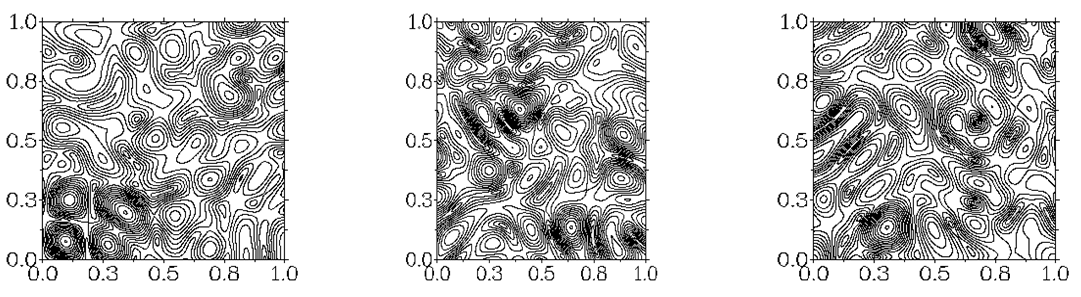
\includegraphics[width=\textwidth]{fig1}
\caption{Contour plots of three multiextremal functions from the test optimization problem family} 
\label{fig:1}
\end{figure}

In \cite{c9}, the proposed approach using the min-max scalarization scheme was compared with the well-known multicriteria optimization methods:
\begin{itemize}
	\item The Monte-Carlo (MC) method, where the trial points are selected within the search domain $D$ randomly and uniformly,
	\item The genetic algorithm SEMO from the PISA library,
	\item The non-uniform coverage (NUC) method,
	\item The bi-objective Lipschitz optimization (BLO) method.
\end{itemize}

In this paper, the efficiency of the proposed approach is compared with other scalarization schemes: the method of successive concessions and the reference point method.

In order to draw more justified conclusions on the efficiency of the developed approach, we solved 100 multicriteria problems formed using the multiextremal functions of the family (\ref{eq:20}). To solve each problem, a total of 50 different coefficients $\alpha$ of the convolutions (\ref{eq:4})-(\ref{eq:6}) were used. The values of the coefficient $\alpha$ are uniformly distributed within the interval $[0,1]$. The parameter values in our experiments were taken as follows: the reliability parameter $r=2,3$, the required accuracy $\varepsilon = 0,01$. All the results presented below were averaged over the family of the  problems solved.

In the first experiment, multicriteria problems were solved using all the considered scalarization schemes (\ref{eq:4})-(\ref{eq:6}), for which a set of different scalarization coefficients was taken. The calculations were performed without using the accumulated search information $A_k$ from (\ref{eq:12}). The numerical results are shown in Table \ref{tab:1}, where the columns labeled ''K'' contain the average number of iterations; in the columns labeled as ''S'', the achieved speedup of the parallel computations is shown. As follows from the presented results of our experiments, the parallel algorithm MPGSA based on the MGGSA method \cite{c10,c16} showed a high efficiency. When employing 16 cores, the speedup was more than 12.5 times for any type of convolutions (\ref{eq:4})-(\ref{eq:6}).

\begin{table}[t]
\caption{Average number of iterations and the speedup of parallel computations when solving a single MCO problem without reusing the search information}\label{tab:1}
\centering
\begin{tabular}{clcclcclcclcclcc}
\hline
           &  & \multicolumn{14}{c}{Number of cores}                                                                                               \\ \cline{3-16}
Convolution&  & \multicolumn{2}{c}{1} &  & \multicolumn{2}{c}{2} &  & \multicolumn{2}{c}{4} &  & \multicolumn{2}{c}{8} &  & \multicolumn{2}{c}{16} \\ \cline{3-4} \cline{6-7} \cline{9-10} \cline{12-13} \cline{15-16} 
           &  & K            & S      &  & K          & S        &  & K          & S        &  & K          & S        &  & K          & S         \\ \cline{1-1} \cline{3-4} \cline{6-7} \cline{9-10} \cline{12-13} \cline{15-16} 
$F_1 (\lambda,y)$ from (\ref{eq:4}) &  & 13 221       & 1      &  & 7 187      & 1,8      &  & 3 456      & 3,8      &  & 1 897      & 7,0      &  & 1 058      & 12,5      \\
$F_2 (\delta,y)$ from (\ref{eq:5})  &  & 16 002       & 1      &  & 9 458      & 1,7      &  & 4 113      & 3,9      &  & 2 356      & 6,8      &  & 1 204      & 13,3      \\
$F_3 (\theta,y)$ from (\ref{eq:6})  &  & 14 041       & 1      &  & 7 866      & 1,8      &  & 3 558      & 3,9      &  & 1 982      & 7,1      &  & 1 068      & 13,2      \\ \hline
\end{tabular}
\end{table}


\begin{table}[t]
\caption{Average number  of iterations and speedup of parallel computations when solving a single MCO problem with the reuse of the search information}\label{tab:2}
\centering
\begin{tabular}{clcclcclcclcclcc}
\hline
           &  & \multicolumn{14}{c}{Number of cores}                                                                                               \\ \cline{3-16}
Convolution&  & \multicolumn{2}{c}{1} &  & \multicolumn{2}{c}{2} &  & \multicolumn{2}{c}{4} &  & \multicolumn{2}{c}{8} &  & \multicolumn{2}{c}{16} \\ \cline{3-4} \cline{6-7} \cline{9-10} \cline{12-13} \cline{15-16} 
           &  & K            & S      &  & K          & S        &  & K          & S        &  & K          & S        &  & K          & S         \\ \cline{1-1} \cline{3-4} \cline{6-7} \cline{9-10} \cline{12-13} \cline{15-16} 
$F_1 (\lambda,y)$ from (\ref{eq:4}) & & 1 193 & 1 & & 595  & 2,0  & & 300 & 4,0  & & 173 & 6,9 & & 103 & 11,5 \\
$F_2 (\delta,y)$ from (\ref{eq:5})  & & 2 021 & 1 & & 934  & 2,2  & & 475 & 4,3  & & 272 & 7,4 & & 147 & 13,7 \\
$F_3 (\theta,y)$ from (\ref{eq:6})  & & 990	  & 1 & & 491  & 2,0  & & 249 & 4,0  & & 145 & 6,8 & & 90	 & 10,9 \\ \hline
\end{tabular}
\end{table}

The results presented in Table \ref{tab:2} show  that by reusing the search information the amount of performed computations can be reduced at least 10-fold.

The efficiency of the developed approach becomes more evident when the obtained reduction of executed optimization iterations is shown in comparison with the initial sequential algorithm, which does not use the search information (Table \ref{tab:3}). As follows from the results of performed experiments, the overall reduction when using 16 computation cores always exceeded 100.

\begin{table}[t]
\caption{Overall reduction of executed iterations provided by using the developed approach for solving a MCO problem}\label{tab:3}
\centering
\begin{tabular}{cccccc}
\hline
                  & \multicolumn{5}{c}{Number of cores} \\ \cline{2-6} 
Convolution       & 1     & 2     & 4    & 8    & 16    \\ \hline
$F_1 (\lambda,y)$ from (\ref{eq:4}) & 11,1  & 22,2  & 44,1 & 76,2 & 127,5 \\
$F_2 (\delta,y)$  from (\ref{eq:5}) & 7,9   & 17,1  & 33,7 & 58,7 & 108,2 \\
$F_3 (\theta,y)$  from (\ref{eq:6}) & 14,2  & 28,6  & 56,3 & 96,3 & 154,9 \\ \hline
\end{tabular}
\end{table}

\section{Conclusion}
In the present paper, a new approach to parallel computations for solving time-consuming multicriteria global optimization problems is presented. This approach is based on various methods for scalarization of vector criteria, on dimensionality reduction with the use of the Peano space-filling curves, and on efficient global search algorithms. 

A novel contribution consists in the development of an approach permitting to use different criteria scalarization schemes with the account of different optimality requirements to desirable decisions. For the scalarization schemes considered, a general method of parallel computations was proposed and the efficiency of the developed approach was evaluated computationally. Our numerical experiments confirmed the efficiency of the proposed approach -- for example, the speedup of parallel computations when using 16 computational cores always exceeded 100.

In further investigations, we intend to perform numerical experiments on parallel solving the multicriteria optimization problems for a larger number of efficiency criteria and for larger dimensionality. Parallel computations on computational nodes with distributed memory can be considered as well.




%
% ---- Bibliography ----
%
% BibTeX users should specify bibliography style 'splncs04'.
% References will then be sorted and formatted in the correct style.
%
% \bibliographystyle{splncs04}
% \bibliography{mybibliography}
%
\begin{thebibliography}{8}


\bibitem{c1} 	Marler, R.T., Arora, J.S.: Multi-Objective Optimization: Concepts and Methods for Engineering. In: VDM Verlag (2009).
\bibitem{c2} 	Ehrgott, M.: Multicriteria Optimization. In: Springer (2nd ed., 2010). 
\bibitem{c3} 	Collette, Y., Siarry, P.: Multiobjective Optimization: Principles and Case Studies (Decision Engineering). In: Springer (2011).
\bibitem{c4} 	Pardalos, P.M., {\v Z}ilinskas, A., {\v Z}ilinskas, J.: Non-Convex Multi-Objective Optimization. In: Springer (2017). 
\bibitem{c5} 	Modorskii, V.Y., Gaynutdinova, D.F., Gergel, V.P., Barkalov, K.A.: Optimization in design of scientific products for purposes of cavitation problems. In: AIP Conference Proceedings, \textbf{1738}, pp. 400013 (2016). \doi{10.1063/1.4952201}
\bibitem{c6} 	Strongin, R.G., Gergel, V.P.: Parallel computing for globally optimal decision making. In: Lecture Notes in Computer Science, \textbf{2763}, pp. 76--88 (2003).
\bibitem{c7} 	Gergel, V., Kozinov, E.: Efficient methods of multicriterial optimization based on the intensive use of search information. In: Springer Proceedings in Mathematics and Statistics, \textbf{197}, pp. 27--45 (2017). \doi{10.1007/978-3-319-56829-4\_3}
\bibitem{c8} 	Barkalov, K., Gergel, V., Lebedev, I.: Solving global optimization problems on GPU cluster. In: AIP Conference Proceedings, \textbf{1738}, pp. 400006 (2016).
\bibitem{c9} 	Gergel, V.P., Kozinov, E.A.: Efficient multicriterial optimization based on intensive reuse of search information. In: J Glob Optim., \textbf{71}(1), pp. 73--90, (2018).
\bibitem{c10}	Strongin, R., Sergeyev, Ya.: Global optimization with non-convex constraints. Sequential and parallel algorithms. In: Kluwer Academic Publishers, Dordrecht (2nd ed. 2013, 3rd ed. 2014).
\bibitem{c11}	Sergeyev Y.D., Strongin R.G., Lera D.: Introduction to global optimization exploiting space-filling curves. In: Springer (2013).
\bibitem{c12}	Zhigljavsky, A., {\v Z}ilinskas, A.: Stochastic Global Optimization. In: Springer (2008).
\bibitem{c13}	Locatelli, M., Schoen, F.: Global Optimization: Theory, Algorithms, and Applications. In: SIAM (2013).
\bibitem{c14}	Floudas, C.A., Pardalos, M.P.: Recent Advances in Global Optimization. In: Princeton University Press (2016).
\bibitem{c15}	Gergel, V.P., Sidorov, S.V.: A Two-Level Parallel Global Search Algorithm for Solution of Computationally Intensive Multiextremal Optimization Problems. In: Parallel Computing Technologies / LNCS, \textbf{9251}, pp. 505--515 (2015).
\bibitem{c16}	Gergel, V., Kozinov, E.: Parallel computing for time-consuming multicriterial optimization problems. In: LNCS, \textbf{10421}, pp. 446--458 (2017). 
\bibitem{c17}	Sergeyev Y.D., Kvasov D.E.: A deterministic global optimization using smooth diagonal auxiliary functions. In: Communications in Nonlinear Science and Numerical Simulation, \textbf{21}(1-3), pp. 99--111 (2015).
\bibitem{c18}	Gergel, V., Grishagin, V., Gergel, A.: Adaptive nested optimization scheme for multidimensional global search. In: JOGO, \textbf{66}(1), pp. 35--51 (2016). 

\end{thebibliography}
\end{document}
